\documentclass[12pt]{article}
\usepackage{amsmath,amssymb,amsfonts}
\usepackage{tikz}
\usepackage[margin=0.5in]{geometry}
\newcommand{\pdata}{p_\mathrm{data}}
\begin{document}
\begin{center}
Name: \rule{3in}{0.4pt} \hfill Total: 15 points
\end{center}

	Let $X \sim \pdata$ be a random variable that takes values on $\{-1,1\}$ with $\pdata(\{-1\}) = \alpha$ and $\pdata(\{1\}) = 1 -\alpha.$ Consider a class of Gaussian model densities $q_\theta = \mathcal{N}(a,b^2),$ where the set of parameters $\theta = (a, b)$ corresponds to the mean and standard deviation of the Gaussian.

\begin{center}
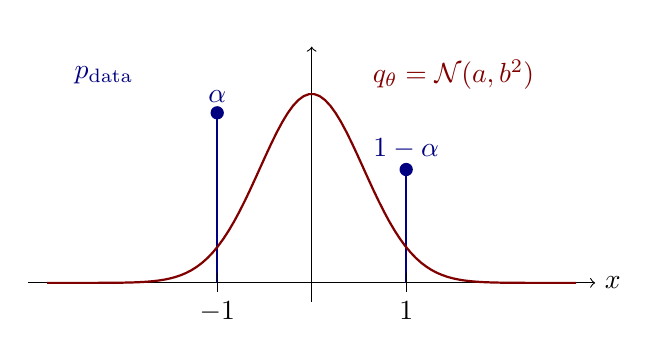
\begin{tikzpicture}[scale=1.2]
    % Axes
    \draw[->] (-3,0) -- (3,0) node[right] {$x$};
    \draw[->] (0,-0.2) -- (0,2.5) node[above] {};

    % p_data: impulses at -1 and 1
    \draw[thick, blue!50!black] (-1,0) -- (-1,1.8) node[above] {$\alpha$};
    \fill[blue!50!black] (-1,1.8) circle (2pt);
    \draw[thick, blue!50!black] (1,0) -- (1,1.2) node[above] {$1-\alpha$};
    \fill[blue!50!black] (1,1.2) circle (2pt);

    % q_theta: Gaussian curve centered!50!black around 0
    \draw[thick, red!50!black, domain=-2.8:2.8, samples=100]
        plot (\x, {2*exp(-(\x)^2/0.6)});

    % Labels
    \node[blue!50!black] at (-2.2,2.2) {$\pdata$};
    \node[red!50!black] at (1.5,2.2) {$q_\theta = \mathcal{N}(a, b^2)$};

    % Tick marks
    \draw (-1,0.1) -- (-1,-0.1) node[below] {$-1$};
    \draw (1,0.1) -- (1,-0.1) node[below] {$1$};
\end{tikzpicture}
\end{center}

\begin{enumerate}
	\item Consider maximizing the likelihood of i.i.d.\ samples $\{x_i\}_{i\in [m]}$ from $\pdata.$ That is, let $$(a^*, b^*) = \theta^* := \arg\max_\theta
\frac{1}{m} \sum_{i=1}^m \log q_\theta(x_i).$$
As $m \to \infty$ and $\alpha = 0$, $q_{\theta^*}$ has zero variance. True or False? Justify your answer. (2 points)

\vfill

\item When $m \to \infty$, for no value of $\alpha \in [0,1]$ does $q_{\theta^*}$ match $\pdata$ exactly. True or False? Justify your answer. (2 points)

\vfill

\newpage

\item Let the source distribution be $\pdata$ and the target be $q_{\theta^*}$. Does an optimal transport map (solution of the Monge problem) exist with the squared Euclidean distance as the cost function, for any $\alpha \in [0,1]$? (1 point)

\vfill

\item The figure below shows the optimal transport map from $q_{\theta^*}$ to $\pdata$ for two different values of $\alpha$ in the left and right plots. Which is greater, $\alpha_1$ or $\alpha_2$, and why? (2 points)
\begin{figure}[h]
\centering
\includegraphics[width=0.9\textwidth]{ot_map_qtheta_to_pdata.pdf}
\caption{Optimal transport map from $q_{\theta^*}$ to $\pdata$.}
\label{fig:ot}
\end{figure}

\vfill

\item In Figure \ref{fig:ot}, the point of discontinuity in the OT map is marked $x(\alpha)$. What is the relationship between $x(\alpha)$ and $\alpha$?
Use the notation $\Phi_{a, b}(x)$ for the CDF of a Gaussian with mean $a$ and variance $b^2.$ (2 points)

\vfill

\newpage
\item The figure below shows the transport plans (solution of the Kantorovich problem) for the source $q_{\theta^*}$ and target $\pdata$ with different values of $\alpha.$ Blue indicates regions of low joint density and red indicates high density. The four values of $\alpha$ used are $\{0.01, 0.2, 0.7, 0.9\}$, but these are not in order! Unscramble them (2 points for correct order, 2 points for explanation):
$$\alpha_1 = \ldots\ldots , \quad \alpha_2 = \ldots\ldots , \quad \alpha_3 = \ldots\ldots , \quad \alpha_4 = \ldots\ldots$$
\begin{figure}[h]
\centering
\includegraphics[width=0.9\textwidth]{transport_plan_contour.pdf}
\caption{Transport plans from $q_{\theta^*}$ to $\pdata$.}
\label{fig:transport}
\end{figure}


\vfill

\item Using the above plots or otherwise, explain for what value of $\alpha$ would $q_{\theta^*}$ be the worst generative model for $\pdata$ in terms of the $W_2$ (Wasserstein-2) metric. (2 points)

\vfill





\end{enumerate}



\end{document}
